
\section{\rqone}
\label{rq1:method}
This research question investigates whether we can artificially generate program variants for \wasm. We use CROW to generate variants from an original program, written in C/C++ in the case of the \corpusrosetta corpus and LLVM bitcodes in the case of \corpussodium and \corpusqrcode. 
In \autoref{diagrams:protocol:rq1} we simplify the workflow to generate \wasm program variants. We pass each function of the corpora to CROW. To answer RQ1, we study the outcome of this pipeline, the generated variants. 


\begin{figure}[h]
    \centering
    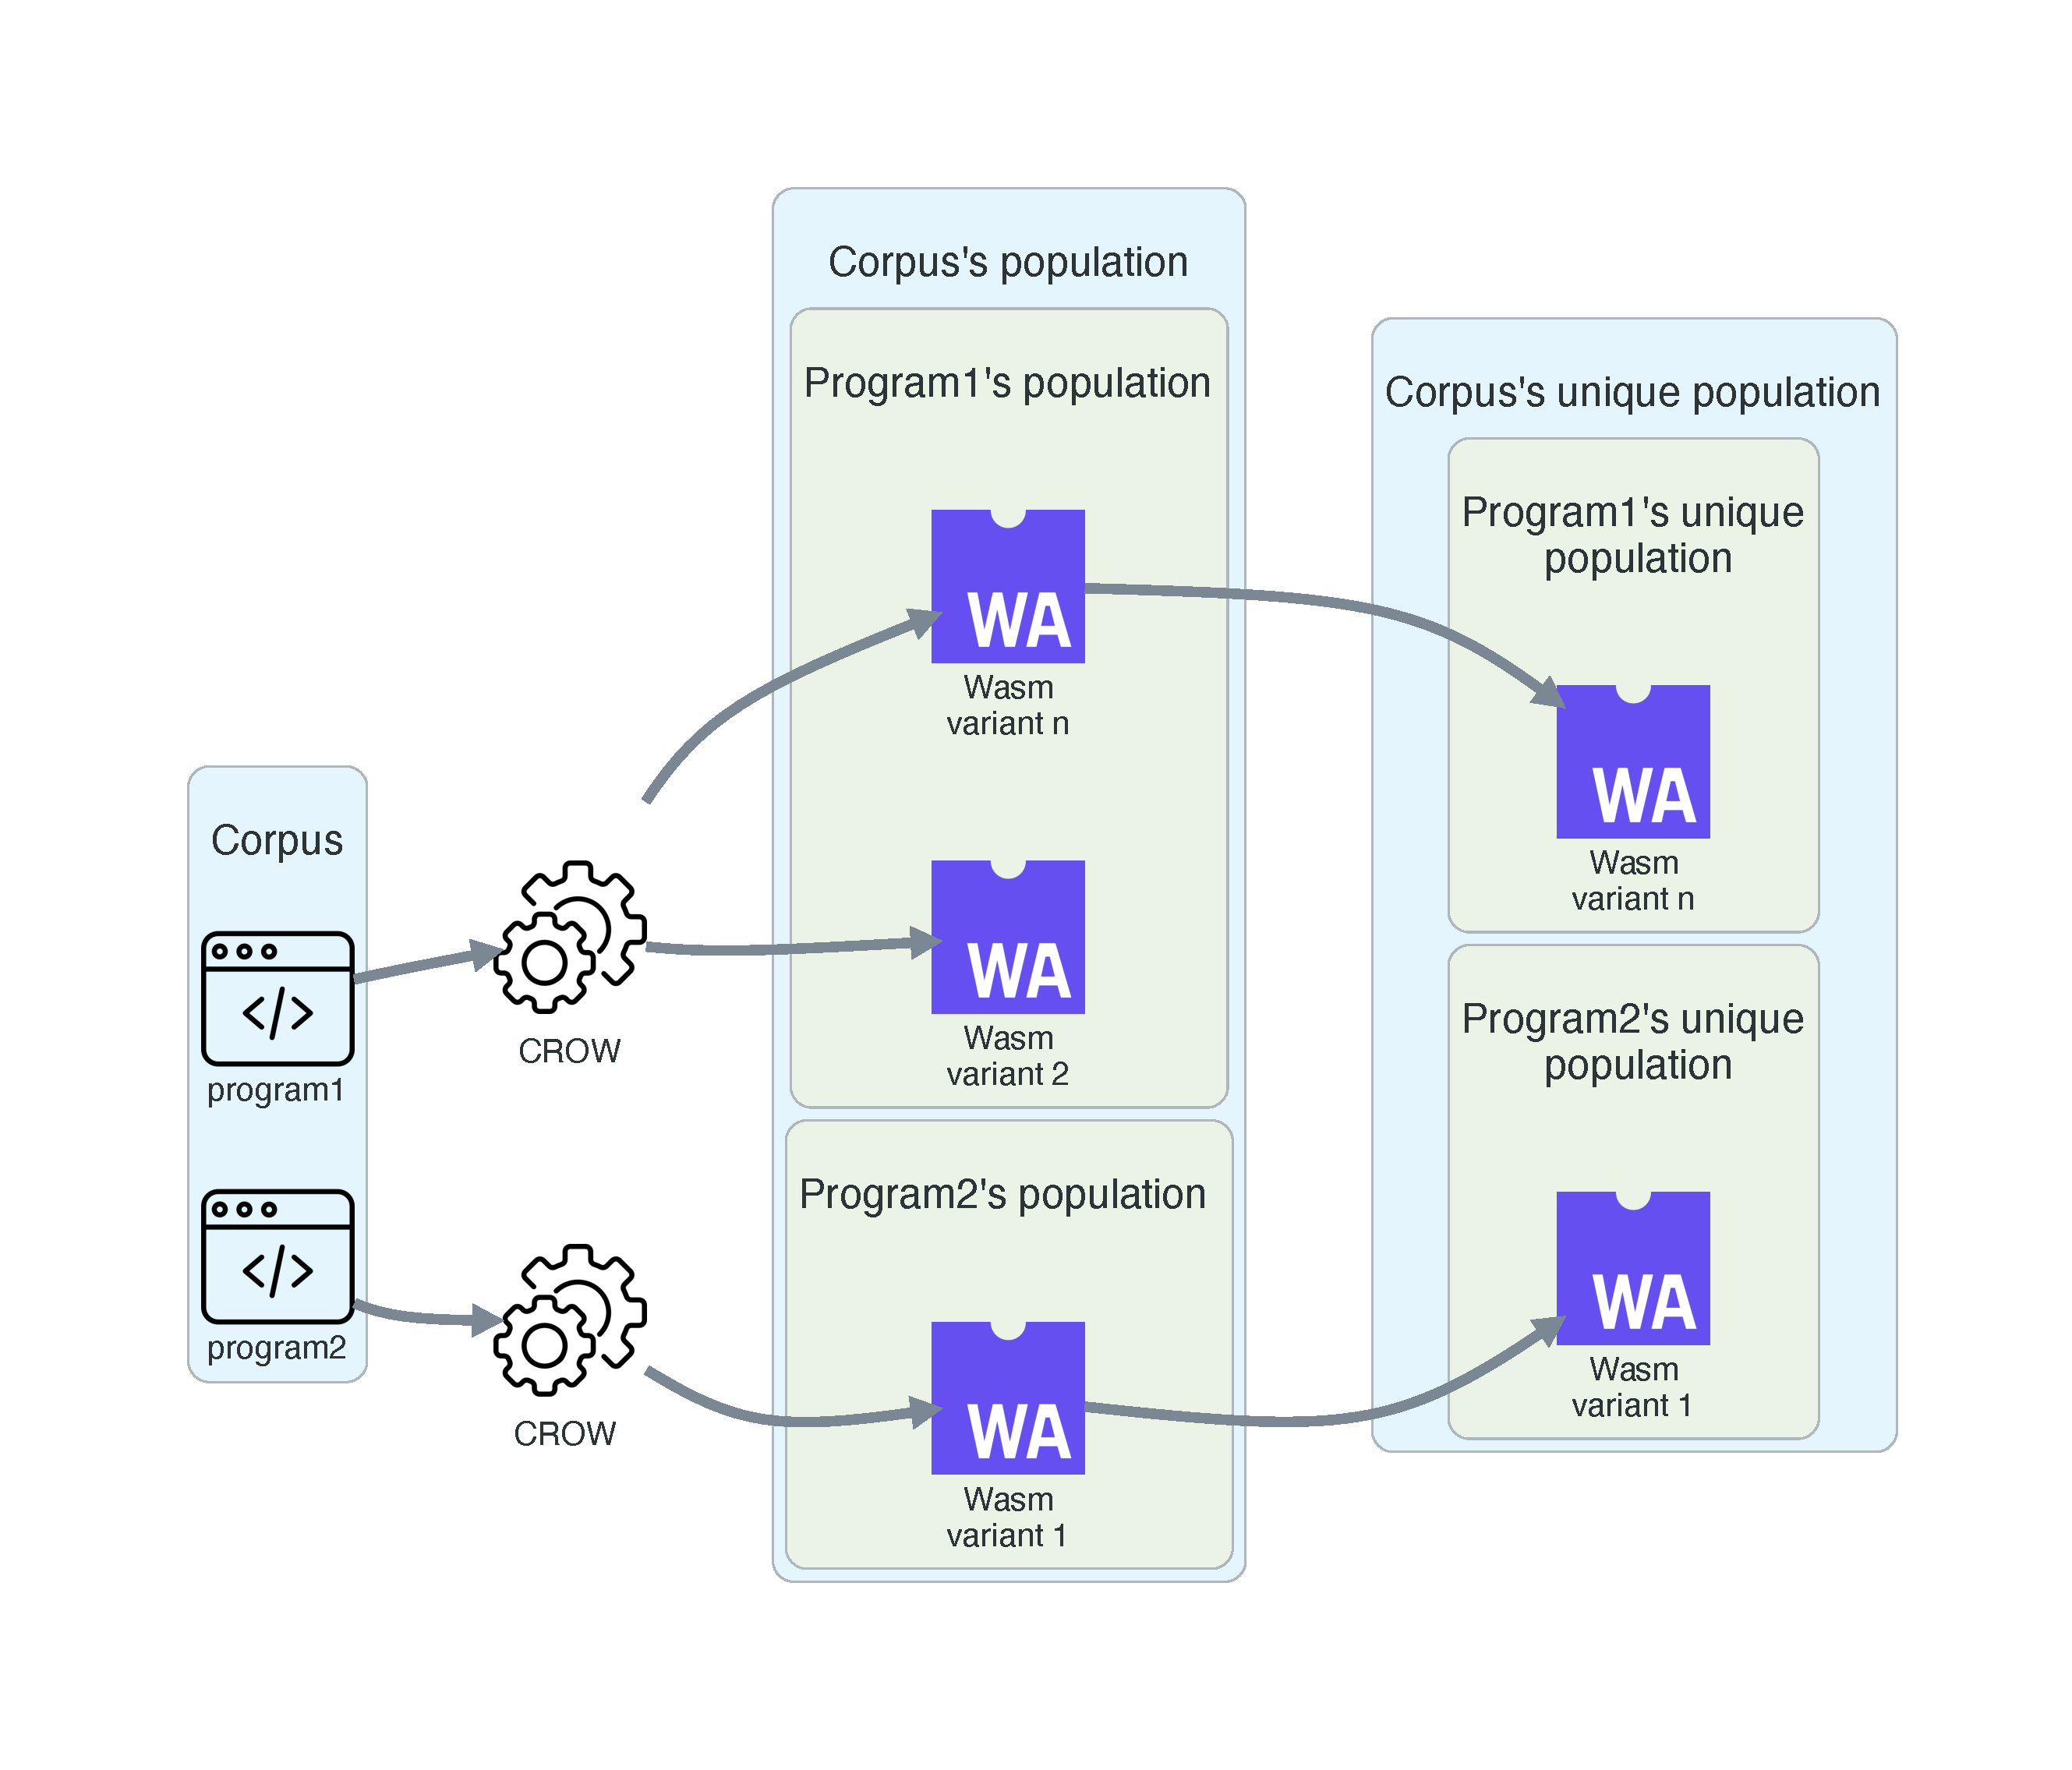
\includegraphics[height=2.4in]{diagrams/Rq1.pdf}
    \caption{The program variants generation for RQ1.}
    \label{diagrams:protocol:rq1}
\end{figure}


\subsection*{Metrics}

To assess our approach's ability to generate \wasm binaries that are statically different, we compute the number of unique variants for each original function of each corpus. 

\begin{metric}{Population size $S(P)$:}\label{metric:md5sum}
    Given a program P and its generated variants $V$, the population size metric is defined as.\\
    $$
        S(P)=|V|
    $$

    Notice that, the variant population includes P as an instance.
\end{metric}

A program and its variants compose what we call a program's population. Notice that all proposed metrics over programs and their variants make sense only at the population level. Therefore, we compare semantically equivalent programs from the same population.

\subsection*{Protocol}
To generate program variants, we mainly synthesize program variants with an enumerative strategy, checking each synthesis for equivalence modulo input \cite{Li2018} against the original program. An enumerative synthesis is a brute-force approach to generate program variants. With a maximum number of instructions, it constructs and checks all possible programs up to that limit. For a simplified instance, with a maximum code size of 2 instructions in a programming language with $L$ possible constructions, an enumerative synthesizer builds all $L\times L$ combinations finding program variants. For obvious reasons, this space is nearly impossible to explore in a reasonable time as soon as the limit of instructions increases.
Therefore, we use two parameters to control the size of the search space and hence the time required to traverse it.
On the one hand, one can limit the size of the variants. On the other hand, one can limit the set of instructions used for the synthesis. In our experiments for RQ1, we use all the $60$ supported instructions in our synthesizer.


The former parameter allows us to find a trade-off between the number of variants that are synthesized and the time taken to produce them. For the current evaluation, given the size of the corpus and the properties of its programs, we set the exploration time to 1 hour maximum per function for \corpusrosetta. In the cases of \corpussodium\ and\ \corpusqrcode, we set the timeout to 5 minutes per function. The decision behind the usage of lower timeout for \corpussodium
and \corpussodium is motivated by the properties listed in \autoref{table:corpora}. The latter two corpora are remarkably larger regarding the number of instructions and functions count. 

We pass each of the $303 + \libsodiumfunctions + \qrcodefunctions$ functions in the corpora to CROW, as \autoref{diagrams:protocol:rq1} illustrates, to synthesize program variants. Finally, we calculate \autoref{metric:md5sum} for each program's population and conclude by answering RQ1.
